% 01-prologue/slides.tex, v. 1 (21/12/12)
% companion files to "Language and Computers"
% Dickinson, Brew, & Meurers (2013)

\documentclass{beamer}

\usepackage{graphicx}
\usepackage{tikz}

\usetikzlibrary{positioning,shapes,arrows,automata}
\def\dx{1cm} \def\dy{1.5cm}
\tikzstyle{state}=[draw,ellipse]

\definecolor{links}{HTML}{2372CC}
\hypersetup{colorlinks,linkcolor=,urlcolor=links}
\parskip=15pt

\newcommand{\newState}[4]{\node[state,#3](#1)[#4]{#2};}
\newcommand{\newTransition}[4]{\path[->] (#1) edge [#4] node {#3} (#2);} 
\usepackage{forest,adjustbox}
\useforestlibrary{linguistics}
\forestapplylibrarydefaults{linguistics}

\title{Introdução a NLP e IR}
\author{Alexandre Rademaker\thanks{Olga Zamaraeva, University of Washington}}
\institute{FGV/EMAp}
\subtitle{Morphology and Finite State Transducers}

\begin{document}

\begin{frame}
  \maketitle
\end{frame}


\section{Morphology and Phonology}

\begin{frame}{Morphology and Phonology}

  \begin{itemize}
  \item Morphology is the study of decomposing words
    \begin{itemize}
    \item {\it Kim sleep-s.}
    \item {\it Kim is sleep-ing.}
    \end{itemize}
  \item Phonology is the study of sound realization based on {\bf environment}
  \item Morphology and Phonology are complex fields
  \item For our purposes, we will look at their simplified versions (mostly just Morphology)
  \item ...in the space of regular languages and FSM
  \end{itemize}
\end{frame}


\begin{frame}{Morphology}
  \begin{itemize}
  \item Lexicon (stems)
  \item affixes:
    \begin{itemize}
    \item prefix {\it {\bf un-}cover}
    \item suffix {\it cover-{\bf ed}}
    \item infix {\it vi{\bf n}co} (Latin, ``I win'', basic root ``vic'')
    \item circumfix {\it {\bf ge-}berg{\bf -te}} (Dutch, ``mountain range'', from ``berg'', mountain)
    \end{itemize}
  \item \href{https://en.wikipedia.org/wiki/Nonconcatenative_morphology}{Templatic morphology}
  \item \href{https://en.wikipedia.org/wiki/Isolating_language}{Isolating languages}
  \item \href{https://en.wikipedia.org/wiki/Fusional_language}{Fusion}
  \item \href{https://en.wikipedia.org/wiki/Agglutinative_language}{Agglutinating}
  \end{itemize}
\end{frame}

% word formation : derivation vs inflection vs compostion

\begin{frame}{Morphological classes}

  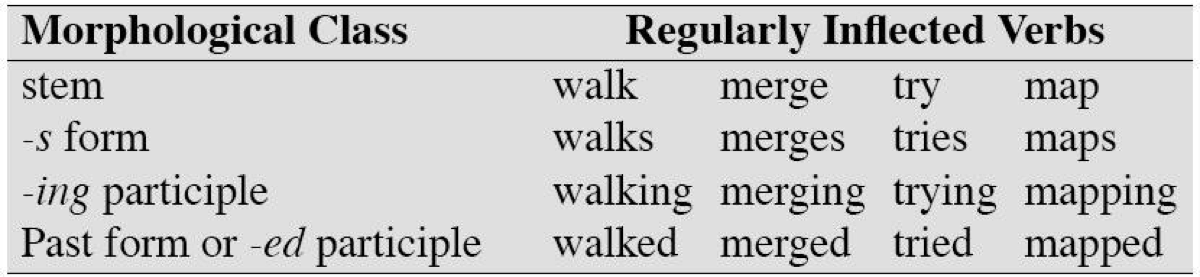
\includegraphics[width=.8\textwidth]{figures/morph-class-reg}

  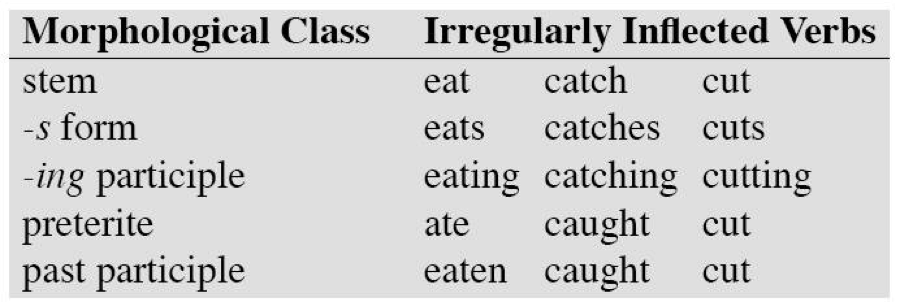
\includegraphics[width=.8\textwidth]{figures/morph-class-irreg}
\end{frame}


\begin{frame}
\frametitle{Morphologically rich languages: Agglutination}
\small
\begin{tabular}{l|l}
Turkish & English\\
\hline
muvaffak & successful \\
muvaffak-iyet & success\\ 
muvaffak-iyet-siz & unsuccessful (without success) \\
muvaffak-iyet-siz-les & to become unsuccessful \\
muvaffak-iyet-siz-les-tir & to make one unsuccessful \\
muvaffak-iyet-siz-les-tiri-ci & maker of unsuccessful ones \\
muvaffak-iyet-siz-les-tiri-ci-les & to become a maker of unsuccessful ones \\
muvaffak-iyet-siz-les-tiri-ci-les-tir & to make one a maker of unsuccessful ones \\
... & ... \\
\end{tabular}

{\tiny
  muvaffakiyetsizlestiricilestiriveremeyebileceklerimizdenmissinizcesine
  \\ like you would be from those we can not easily make a maker of
  unsuccessful ones}

\url{https://www.rabiaergin.com/turkish-morphology.html}
\end{frame}

\begin{frame}{Morphologically rich languages: Fusion}
\begin{small}
\begin{tabular}{l|l}
Russian & English\\
\hline
zl{\bf o} & evil (noun:neut, nom, sg)\\
zl{\bf a} & evil (noun:neut, gen, sg)\\
zl{\bf oj} & evil (adj., masc, nom, sg)\\
zl{\bf aja} & evil (adj., fem, nom, sg) \\
zl{\bf ogo} & evil (adj., masc, gen, sg) \\
zl{\bf ost} & anger, malevolence (noun:fem,nom,sg)\\
zlost{\bf i} & anger, malevolence (noun:fem,gen,sg)\\
zlost{\bf n-ogo} & evil,malignant (adj, masc, gen, sg)\\
zlostn{\bf ost} & evil, malignancy (noun:fem, nom, sg)\\
zlostnost{\bf i} & evil, malignancy (noun:fem, gen, sg)\\
\hline
\end{tabular}
\end{small}
\end{frame}


\begin{frame}{Fusion vs. Agglutination}
  Fusion:
  \begin{itemize}
  \item one affix can combine several features (e.g. Case, Number, Gender)
  \item affixes tend to {\it fuse} with each other and with the base, forming a new base
  \item once the affix fuses, it ``no longer means what it used to''
  \item common in Indo-European languages
  \end{itemize}

  Agglutination
  \begin{itemize}
  \item one affix typically ``means'' one feature
  \item affixes maintain their ``meaning'' in long words
  \item common in Turkic languages
  \end{itemize}
\end{frame}


\begin{frame}{Derivational morphology}
  \begin{itemize}
  \item e.g., {\it un-}, {\it re-}, {\it anti-}, {\it -ism}, {\it -ist} etc
  \item broad range of semantic possibilities, may change part of speech
  \item indefinite combinations\\
    e.g., {\it antiantidisestablishmentarianism}\\
    {\it anti-anti-dis-establish-ment-arian-ism}
  \item generally semi-productive: e.g., {\it escapee}, {\it textee}, {\it ?dropee},
    {\it ?snoree}, {\it *cricketee} (* and ?)
  \item zero-derivation: e.g. {\it tango}, {\it waltz}
  \end{itemize}
\end{frame}

\begin{frame}{Internal structure and ambiguity}
  \emph{Morpheme ambiguity} stems and affixes may be individually
  ambiguous: e.g. {\it dog} (noun or verb), {\it +s} (plural or
  3persg-verb)

  \emph{Structural ambiguity}: e.g., {\it shorts} or {\it short -s}\\
  {\it unionised} could be {\it union -ise -ed} or {\it un- ion -ise
    -ed}

  \emph{Bracketing}: {\it un- ion -ise -ed}

  \begin{itemize}
  \item {\it un- ion} is not a possible form, so not {\it ((un- ion) -ise) -ed}
  \item {\it un-} is ambiguous:
    \begin{itemize}
    \item  with verbs: means `reversal' (e.g., {\it untie})
    \item  with adjectives: means `not' (e.g., {\it unwise, unsurprised})
    \end{itemize}
  \item therefore {\it (un- ((ion -ise) -ed))} 
  \end{itemize}
\end{frame}


\begin{frame}{Using morphological processing in NLP}
  \begin{itemize}
  \item compiling a \emph{full-form} lexicon
  \item recognizing and normalizing mini-formal languages (e.g. dates)
  \item \emph{stemming} for IR (not linguistic stem)
  \item \emph{lemmatization} (often inflections only): finding stems
    and affixes as a precursor to parsing.  \emph{morphosyntax}:
    interaction between morphology and syntax
\end{itemize}
\end{frame}


\begin{frame}{Spelling rules}
  \begin{itemize}
  \item English morphology is essentially concatenative
  \item irregular morphology --- inflectional forms have
    to be listed
  \item regular phonological and spelling 
    changes associated with affixation, e.g.
    \begin{itemize}
    \item {\it -s} is pronounced differently
      with stem ending in {\it s}, {\it x}
      or {\it z}
    \item spelling reflects this with the addition
      of an {\it e} ({\it boxes} etc) 
    \end{itemize}
    \emph{morphophonology}
  \item in English, description is independent of particular stems/affixes
  \end{itemize}
\end{frame}


\begin{frame}[fragile]{Lexical requirements for morphological processing}
  \begin{itemize}
  \item affixes, plus the associated information conveyed by the
    affix
    \begin{verbatim}
      ed PAST_VERB
      ed PSP_VERB 
      s PLURAL_NOUN
    \end{verbatim}
  \item irregular forms, with associated information similar to that for affixes
    \begin{verbatim}
      began PAST_VERB begin
      begun PSP_VERB begin
    \end{verbatim}
  \item stems with syntactic categories (plus more)
  \end{itemize}
\end{frame}


\begin{frame}{Morphological parsing}
  \begin{itemize}
  \item Accept/reject strings consisting of morphemes
    \begin{itemize}
    \item E.g.\ for spell-checking
    \item What about just encoding the lexicon as a list of words?
    \end{itemize}
  \item Map strings to bundles/sequences of linguistic features
  \item Morphological analysis for research support
    \begin{itemize}
    \item A parser as a {\it hypothesis}
    \item Build a parser based on your current understanding of what the language does
    \item Then run it over a corpus of words, see how much it actually parsed and where and why it broke
    \end{itemize}
  \end{itemize}
  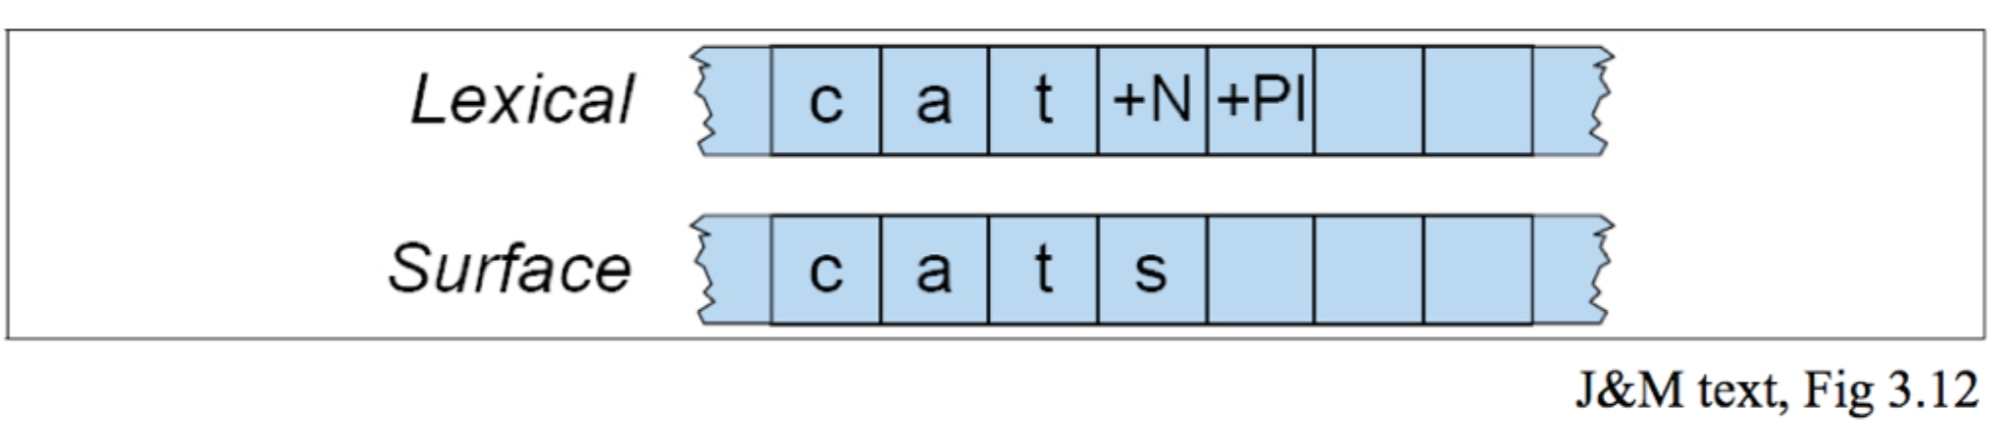
\includegraphics[width=\textwidth]{figures/cats}
\end{frame}


\begin{frame}{FSA for morphological parsing}
  \begin{itemize}
  \item Create FSAs for classes of word stems (word lists).
  \item Create FSA for affixes using word classes as stand-ins for the stem word lists.
  \item Concatenate FSAs for stems with FSAs for affixes.
  \end{itemize}
  
\includegraphics[width=\textwidth]{figures/3-3}
\end{frame}


\begin{frame}{Finite State Transducers}

  Analyzing ({\it parsing}) a word morphologically:
  
  {\it cat} is {\it cat [+N, +SG]},
  
  {\it cats} is {\it cat [+N, +PL]}

  \vspace{0.5cm}

  \centering
  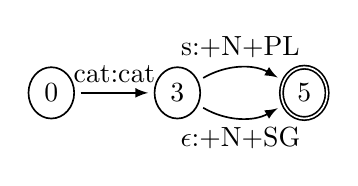
\begin{tikzpicture}[node distance=\dy and \dx,
    >=latex,shorten >=2pt,shorten <=2pt,auto,semithick]
    \newState{S}{$0$}{}{}
    \newState{q3}{$3$}{right=of S}{}
    \newState{q5}{$5$}{right=of q3}{accepting}
    \newTransition{S}{q3}{cat:cat}{}
    \newTransition{q3}{q5}{s:+N+PL}{above, bend left}
    \newTransition{q3}{q5}{$\epsilon$:+N+SG}{below,bend right}
  \end{tikzpicture}
\end{frame}

\begin{frame}{FST and FSA}
  \begin{itemize}
  \item FSA define regular expressions
  \item FST define {\bf regular relations}
  \item FST use two alphabet sets
  \item The {\bf transition} function relates input to states
  \item the {\bf output} function relates input to output
  \end{itemize}
\end{frame}

\begin{frame}{Visualizing FST}
  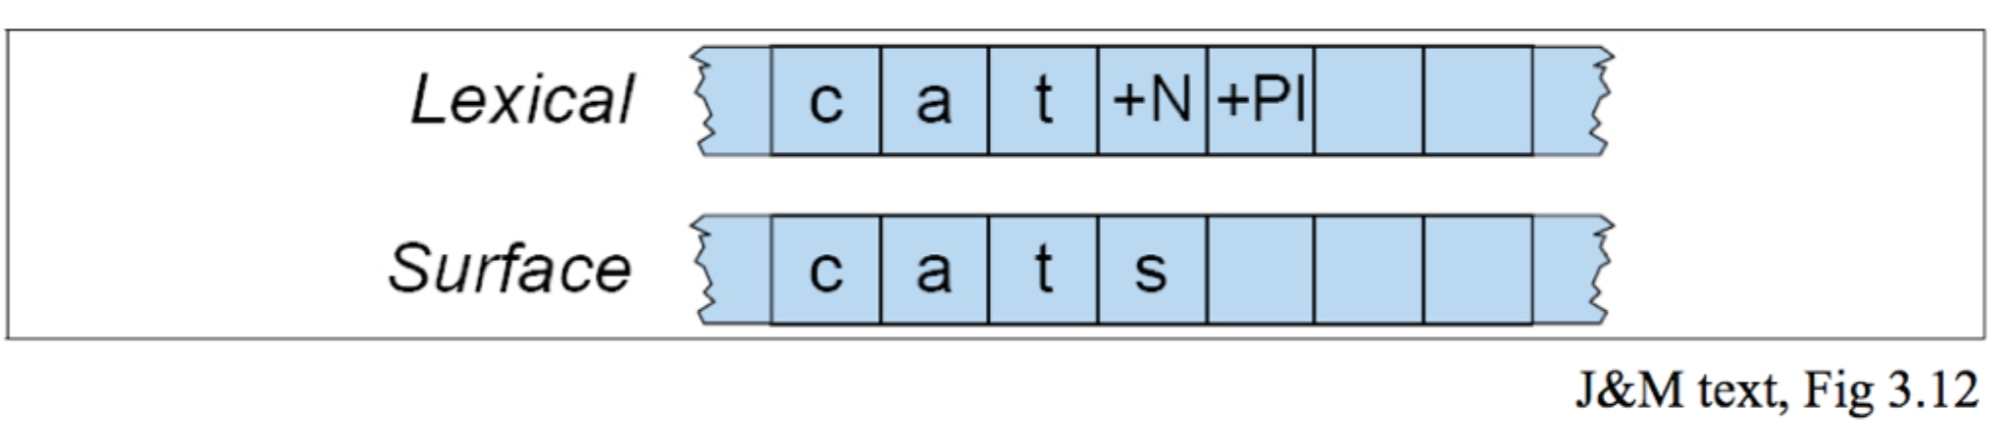
\includegraphics[width=\textwidth]{figures/cats}

  upper and lower tapes
\end{frame}

\begin{frame}{Regular relations}
  \begin{itemize}
  \item Regular language: a set of strings
  \item Regular relation: a set of {\bf pairs} of strings:
    \begin{itemize}
    \item E.g., Regular relation = \{a:1, b:2, c:2\}
    \item Input $\sum$ = \{a,b,c\} Output =\{1, 2\}
    \end{itemize}
  \end{itemize}
  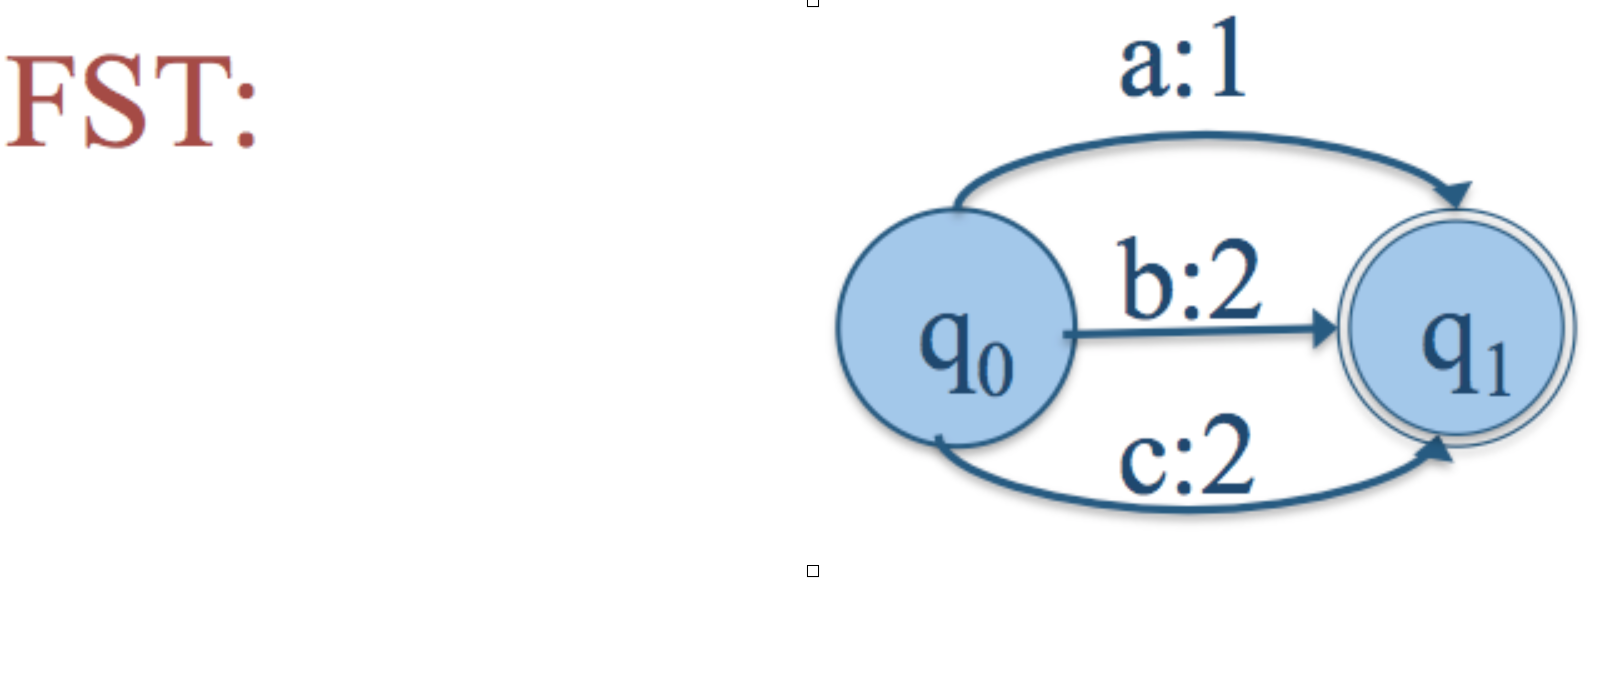
\includegraphics[width=\textwidth]{figures/fst1}
\end{frame}

\begin{frame}{FST conventions}
  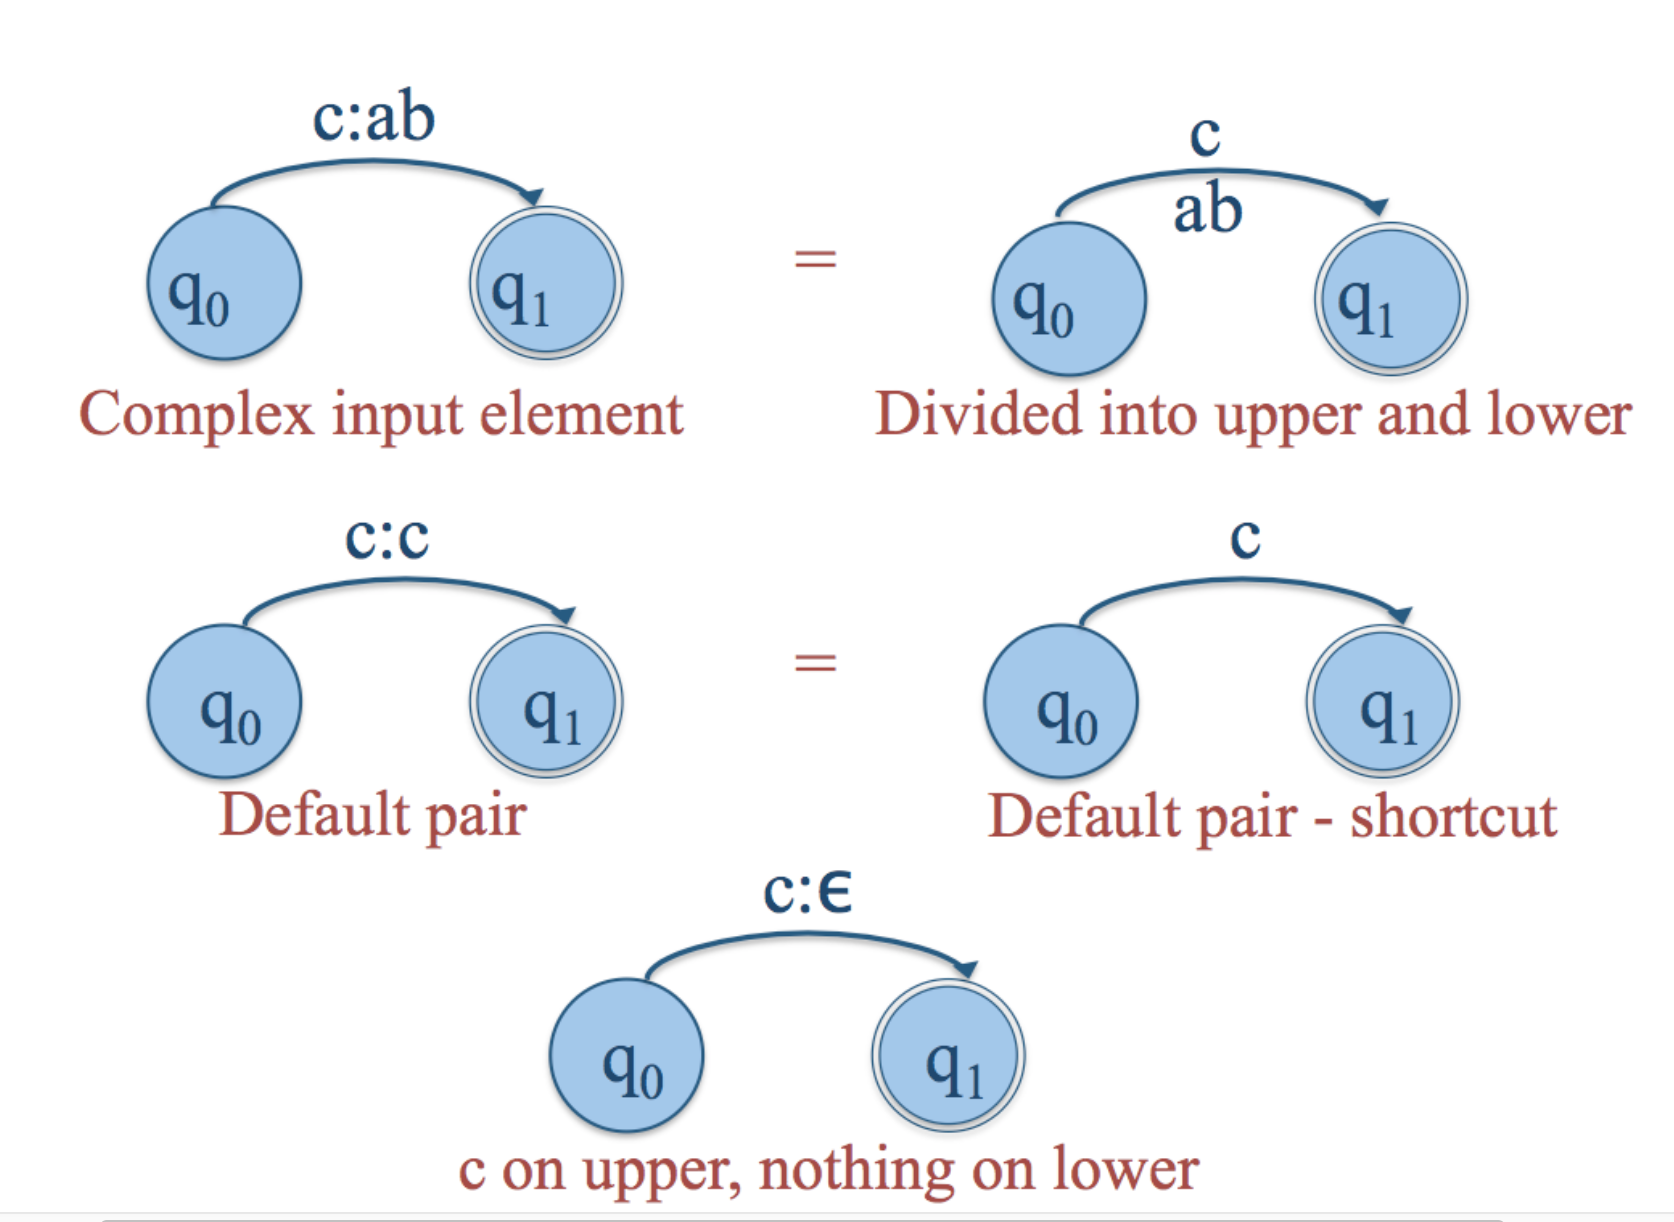
\includegraphics[width=\textwidth]{figures/fst-conventions}
\end{frame}

\begin{frame}{Inversion}
  \begin{itemize}
  \item Inversion of an FST switches input and output labels
  \item Thus we can turn a {\it parser} into a {\it generator}
  \item Parsing:
    \begin{itemize}
    \item Input: cat
    \item Output: cat+N+SG
    \end{itemize}
  \item Generating:
    \begin{itemize}
    \item Input: cat+N+PL
    \item Output: cats
    \end{itemize}
  \end{itemize}

  \begin{center}
    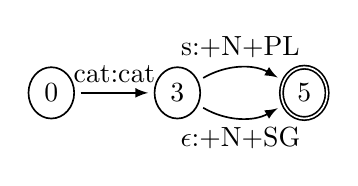
\begin{tikzpicture}[node distance=\dy and \dx,
      >=latex,shorten >=2pt,shorten <=2pt,auto,
      semithick  %semithick, thick, thin semithick
      ]
      \newState{S}{$0$}{}{}
      \newState{q3}{$3$}{right=of S}{}
      \newState{q5}{$5$}{right=of q3}{accepting}
      \newTransition{S}{q3}{cat:cat}{}
      \newTransition{q3}{q5}{s:+N+PL}{above, bend left}
      \newTransition{q3}{q5}{$\epsilon$:+N+SG}{below,bend right}
    \end{tikzpicture}
  \end{center}
  
  \begin{center}
    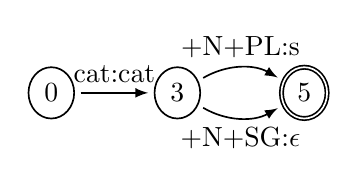
\begin{tikzpicture}[node distance=\dy and \dx,
      >=latex,shorten >=2pt,shorten <=2pt,auto,
      semithick  %semithick, thick, thin semithick
      ]
      \newState{S}{$0$}{}{}
      \newState{q3}{$3$}{right=of S}{}
      \newState{q5}{$5$}{right=of q3}{accepting}
      \newTransition{S}{q3}{cat:cat}{}
      \newTransition{q3}{q5}{+N+PL:s}{above, bend left}
      \newTransition{q3}{q5}{+N+SG:$\epsilon$}{below,bend right}
    \end{tikzpicture}
  \end{center}
\end{frame}


\begin{frame}{Composition}
  \begin{itemize}
  \item example: 
    \begin{itemize}
    \item T1 = \{a:1\}
    \item T2 = \{1:one\} 
    \item T1$\cdot$ T2 = \{a:one\} 
    \item T2(T1(a)) =one
    \end{itemize}
  \item Note that order matters: T1(T2(a)) $\neq$ one
  \item Take a minute: what is T1(T2(a))?
  \item Composition is used for complex morphological analysis (e.g.\ semitic languages)
  \end{itemize}
  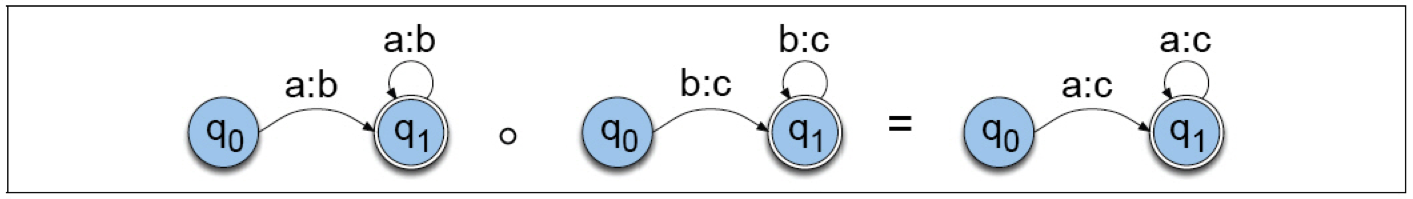
\includegraphics[width=\textwidth]{figures/3-9-composition}
\end{frame}


\begin{frame}{Morphological parsing with FST}
  \begin{itemize}
  \item A very influential approach since Koskenniemi (1983)
  \item AKA ``two-level morphology''
  \item an example of a {\it symbolic} approach
  \end{itemize}
\end{frame}

\begin{frame}{Recognizing/analyzing complex words}
  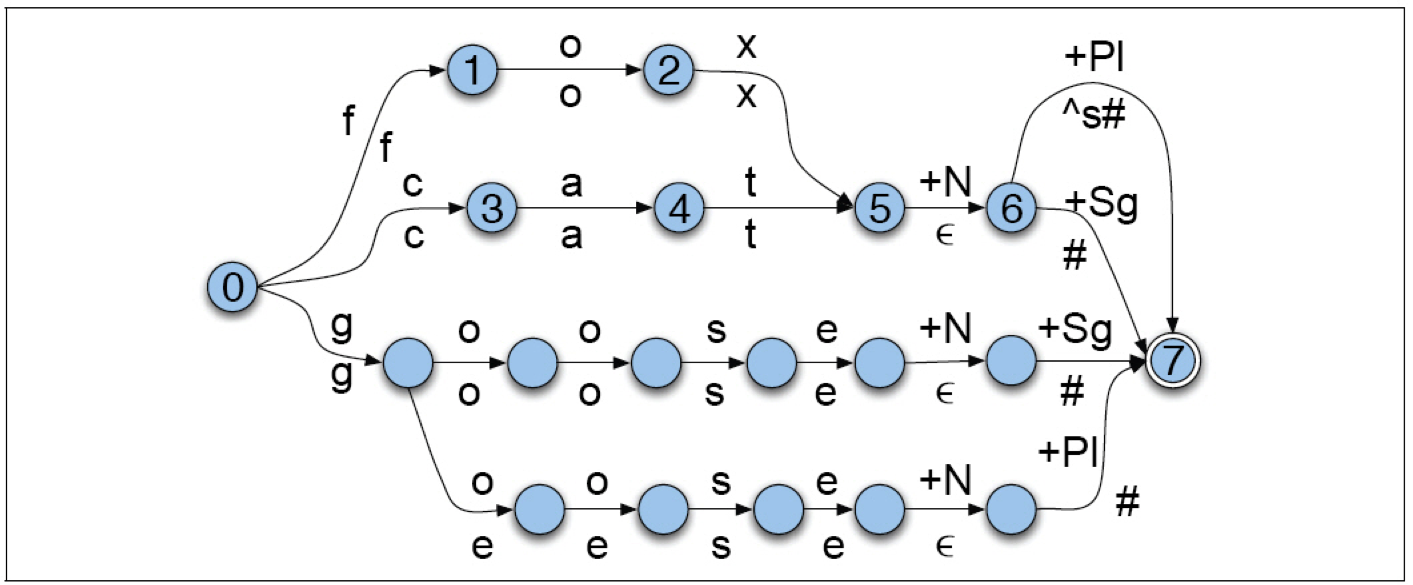
\includegraphics[width=\textwidth]{figures/3-14}

  If I only wanted to {\it recognize}, what would I need?
\end{frame}

\begin{frame}{Recognizing/analyzing complex words}
  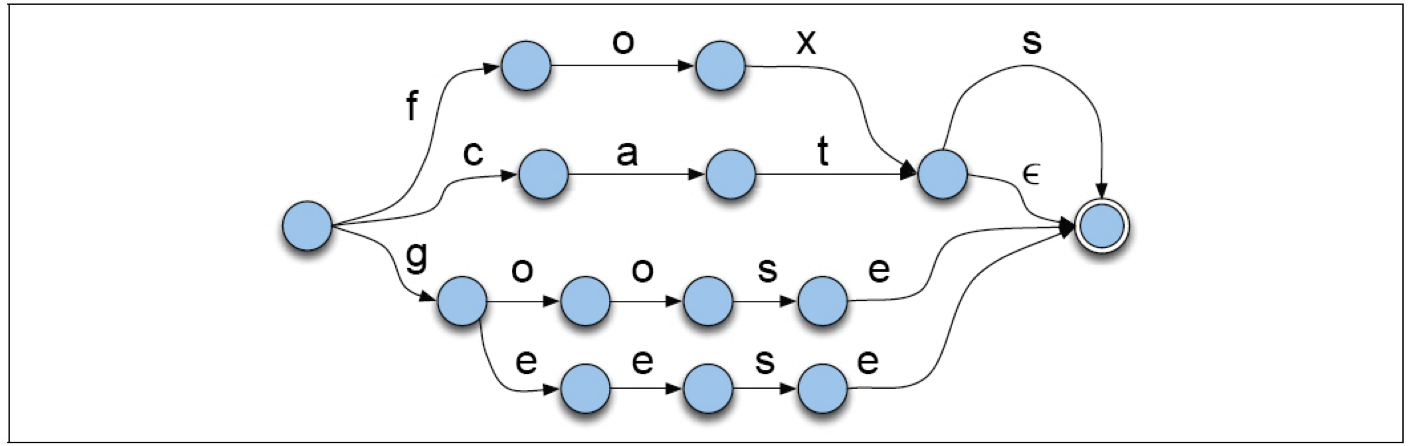
\includegraphics[width=\textwidth]{figures/3-7}

  Just an FSA
\end{frame}

\begin{frame}{Identifying word classes}
  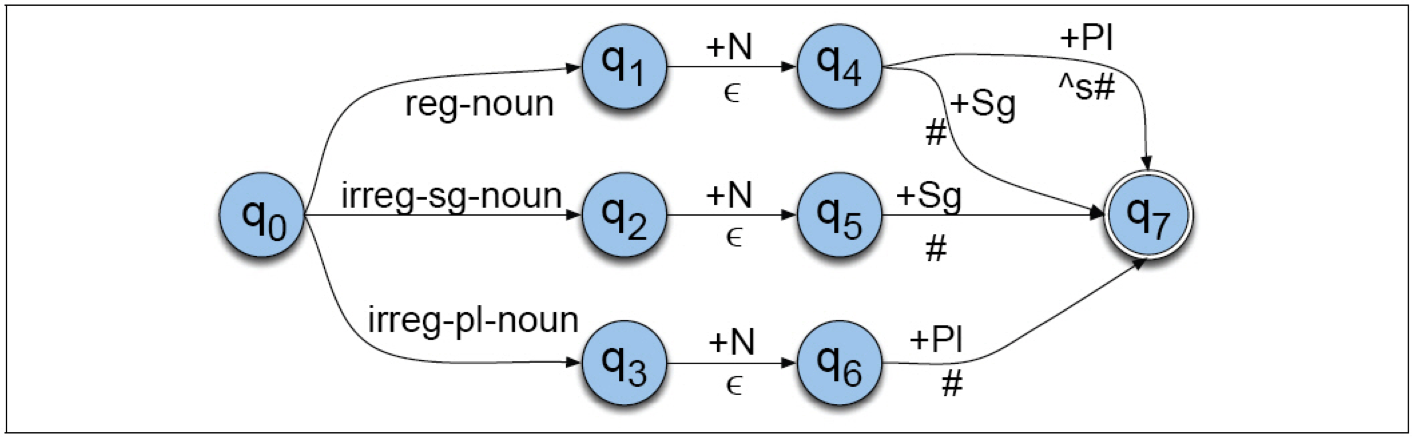
\includegraphics[width=\textwidth]{figures/3-13}
\end{frame}

\begin{frame}{Inflectional classes: Indo-European}
  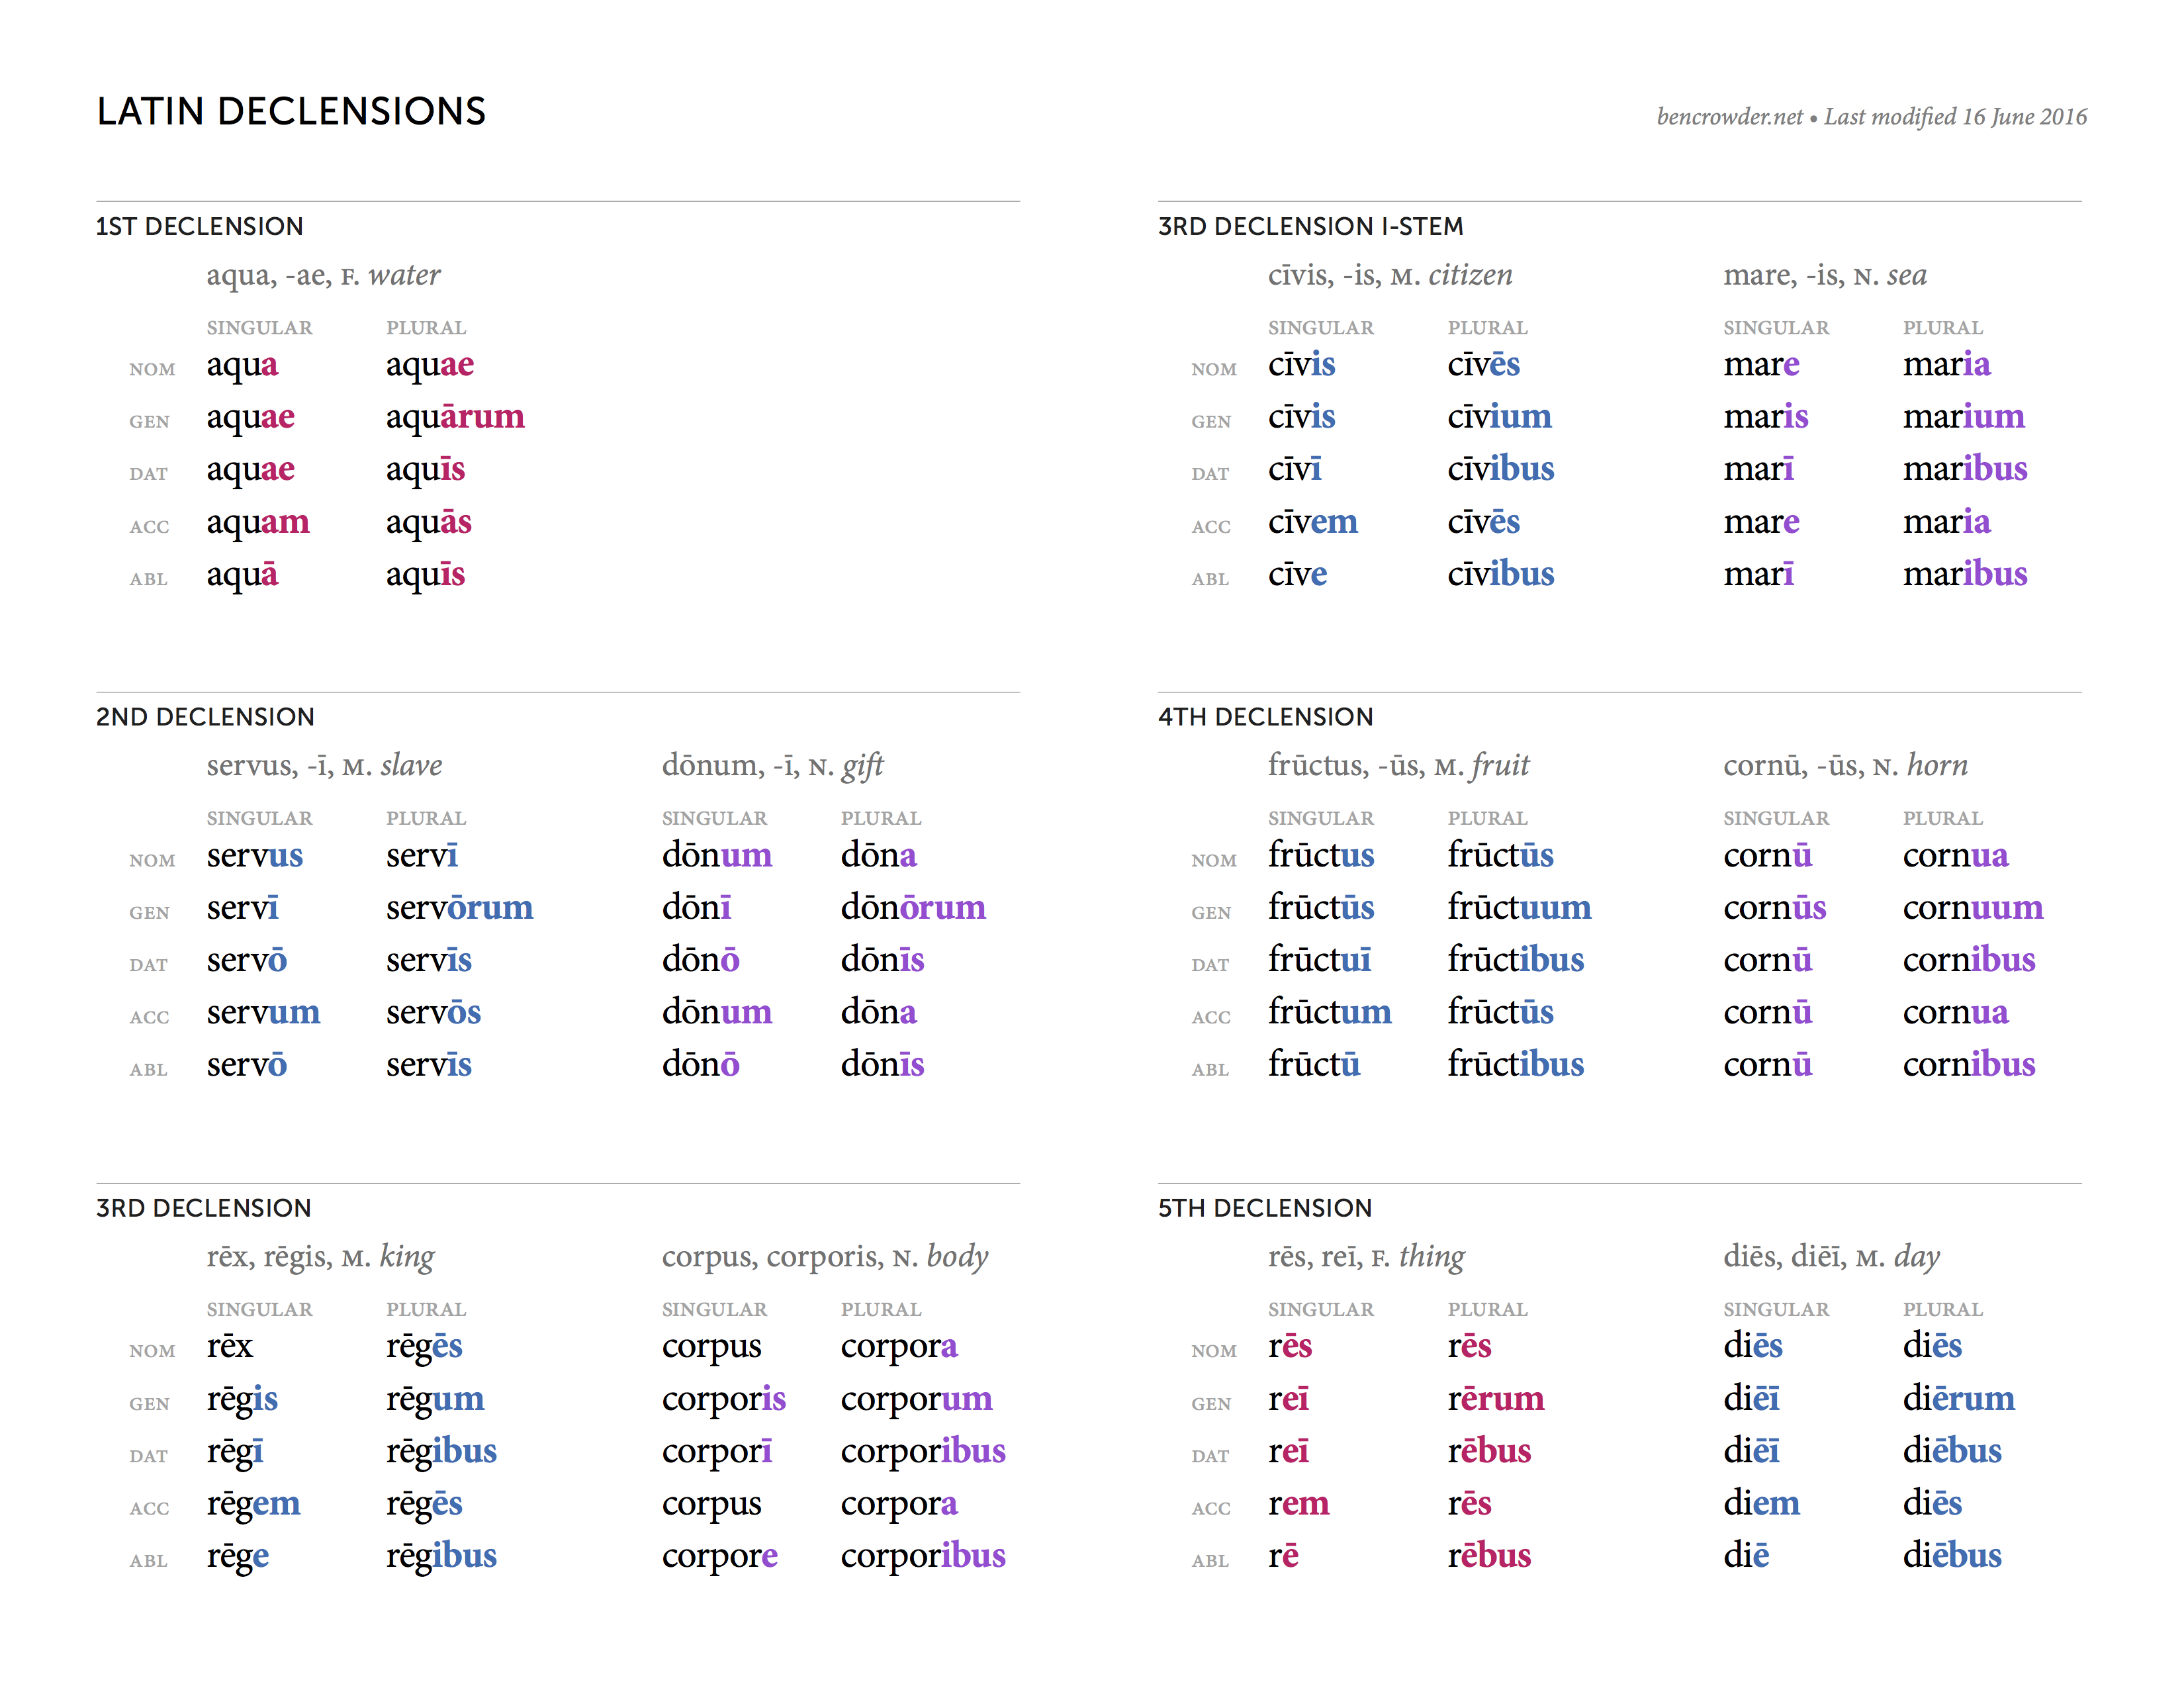
\includegraphics[width=\textwidth]{figures/latin-declensions}
\end{frame}

\begin{frame}{Inflectional classes: Bigger picture}
  \begin{itemize}
  \item Nobody really needs to {\bf look for} inflectional classes in
    IE languages\ldots particularly not in Latin (well-studied) \ldots
  \item But there are many languages in the world for which the exact
    morphological behavior is not yet fully understood
  \item Why is it important that we learn about it and describe it?
  \end{itemize}
\end{frame}

\begin{frame}{Example: Abui [abz] (Alor island in Indonesia)}
  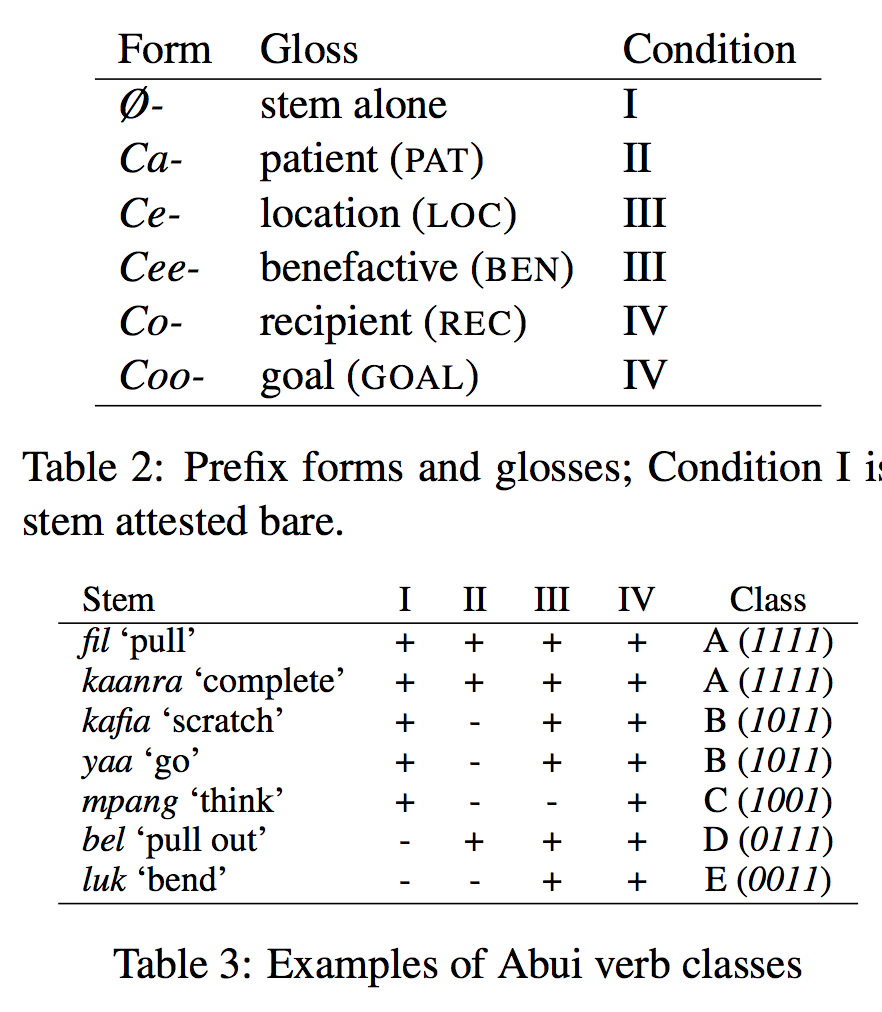
\includegraphics[height=0.8\textheight]{figures/abz}
  
  {\tiny Zamaraeva et al. Computational Support for Finding Word
    Classes: A Case Study of Abui (2017)}
\end{frame}


\begin{frame}{Probabilistic morphological parsing}
  \begin{itemize}
  \item Train a model on a large training corpus
  \item E.g. the corpus contains pairs of surface and underlying strings
    \begin{itemize}
    \item (like that same cats/cat+N+PL pair)
    \end{itemize}
  \item morpheme boundaries can be inferred statistically
  \item Neural nets very successful
  \item Not an option when there is no training data
  \item Other limitations?
  \end{itemize}
\end{frame}

\begin{frame}{Using FSTs}
  \begin{itemize}
  \item FSTs assume \emph{tokenization} (word boundaries) and words
    split into characters.  One character pair per transition!
  \item Analysis: return character list with affix boundaries, so
    enabling lexical lookup.
  \item Generation: input comes from stem and affix lexicons.
  \item One FST per spelling rule: either compile to big FST or run in
    parallel.
  \item FSTs do not allow for internal structure:
    \begin{itemize}
    \item can't model {\it un- ion -ize -d} bracketing.
    \item can't condition on prior transitions, so potential
      redundancy
    \end{itemize}
  \end{itemize}
\end{frame}

\begin{frame}{Foma}
  \begin{itemize}
  \item \url{https://fomafst.github.io/}
  \item Tutorial 1 (basic)
  \item Tutorial 2 (more advanced)
  \end{itemize}
\end{frame}

\begin{frame}{Concluding comments}
  \begin{itemize}
  \item English is an outlier among the world's languages: very
    limited inflectional morphology.
  \item English inflectional morphology hasn't been a practical
    problem for NLP systems for decades.
  \item Limited need for probabilities, small number of possible morphological analyses for a word.
  \item Lots of other applications of finite-state techniques: fast,
    supported by toolkits, good initial approach for very limited
    systems.
  \end{itemize}
\end{frame}


\end{document}

%%% Local Variables:
%%% mode: latex
%%% TeX-master: t
%%% End:
